\documentclass[letterpaper,10pt,draftclsnofoot,onecolumn,]{article}
\usepackage[utf8]{inputenc}
\usepackage[margin=0.75in]{geometry}
\usepackage{pgfgantt}
\usepackage{tikz}
\usepackage{listings}
\usepackage{minted}
\begin{document}
\noindent
\begin{titlepage}
    \begin{center}
        \vspace*{1cm}
        
        \textbf{Gymnastics Scoring Software}
        
        \vspace{0.5cm}
        The purpose of this paper is to give a detailed overview of our current progress and remaining work to be done.
        
        
        \vspace{1.5cm}
        
        \textbf{10.0 Software}
        
        Progress Report\\
        CS 462\\
        Senior Software Engineering Project\\
        Winter 2019
        
        \vspace{8cm}
        Prepared for\\
        Michael Chaplin\\
        
        \vspace{1.5cm}
        Prepared by\\
        Nicholas Giles\\
        Mary Jacobsen\\
        Thomas Huynh\\
        Zech DeCleene
        
        \vspace*{\fill}
        \begin{center}
            \textbf{\large{Abstract}}
        \end{center}
        \normalsize{This document outlines the progress made by 10.0 Software and provides an overview of the system as well as documents the design and functionality of the alpha and beta builds.}
        
    \end{center}
\end{titlepage}

\tableofcontents
\newpage

\begin{center}
\section{Recap}
\end{center}

\subsection{System Purpose}
The system we will be designing is for the scoring of gymnastics meets held in Gill Coliseum. The system will take in, calculate, organize, format, and display scores as well as export and print the scores.

\subsection{System Goals}
The purpose of this system is to provide an improved viewing experience for OSU Gymnastics spectators as well as make the scoring process easier for the judges. The system will be comprised of a web application running on the Gill servers that is accessible by the meet staff to input or adjust scores. The scores will then be formatted to be displayed on the scoreboards inside Gill. The application will be able to format all current data into a score sheet that the user can print out at any time. The system will also comprise of a back-end API with a SQL database running on the Gill servers to store all scoring information.

\subsection{System Overview}
The system is comprised of three main components.
\begin{itemize}
    \item \textbf{Web Application:}
          The Web application's main function will be the user interface which allows the meet staff to add, edit and print scores. The web application will be responsible for formatting and calculating scores then pushing the data to the database and scoreboard.
    \item \textbf{Scoreboard Utilization:}
          Data collected from the web application will be pushed to display up-to-date information on current events of the meet.
    \item \textbf{Database:}
          The database will maintain current and past information. The information will include the teams, judges, athletes, and the scores associated with each athlete and judge.
\end{itemize}

\section{Current Progress}
Currently we are in the process of improving our alpha version and getting it ready for beta. Improvements include changing the structure of the database, client side JavaScript, printing, and security.
\subsection{Alpha}
The alpha version of the software has these features currently implemented:
\begin{enumerate}
    \item Docker containerization
    \item Working MySql database
    \subitem Initially 3 separate files
    \item Working endpoints for /team, /player and /lineup
    \subitem \begin{minted}{mysql}
    #--Example of player-init.sql--
    
    DROP TABLE IF EXISTS `player`;
    CREATE TABLE `player` (
    `id` mediumint(9) NOT NULL AUTO_INCREMENT,
    `playerNum` mediumint(9),
    `name` varchar(255) NOT NULL,
    `team` varchar(255) NOT NULL,
    `vaultScore` DECIMAL(13,10),
    `barsScore` DECIMAL(13,10),
    `beamScore` DECIMAL(13,10),
    `floorScore` DECIMAL(13,10),
    `AAScore` DECIMAL(13,10),
    PRIMARY KEY (`id`),
    KEY `idx_name` (`name`)
    ) ENGINE=InnoDB AUTO_INCREMENT=20 DEFAULT CHARSET=latin1;
    \end{minted}
    \item Functional scoring and lineup pages
    \subitem \begin{minted}{js}
    //--Example of client-side request--
    
    function getTeamData() {
        var url = window.location.origin;
        $.getJSON(url + "/team/teams", (data) => {
            var teams = [];
            console.log(data)
            $.each(data, (key, val) => {
                teams.push("<option value='" + 
                val.teamName + "'>" +
                val.teamName + "</option>");
            });

        $("#team-select").append(teams.join(""));
        });
    }
    \end{minted}
    \subitem \begin{minted}{js}
    //--Example of server-side response--
    
    router.get('/:id', function (req, res, next) {
        console.log(" -- req.params:", req.params.id);
        const mysqlPool = req.app.locals.mysqlPool;
        const id = req.params.id;
        getTeamByID(id, mysqlPool)
        .then((id) => {
          if (id) {
            res.status(200).json(id);
          } else {
              next();
          }
        })
        .catch((err) => {
          res.status(500).json({
            error: "Unable to fetch team.  Please try again later."
          });
        });
    });
    
    function getTeamByID(id, mysqlPool) {
      return new Promise((resolve, reject) => {
        mysqlPool.query('SELECT * FROM team WHERE id = ?', [ id ], function (err, results) {
          if (err) {
            reject(err);
          } else {
            resolve(results[0]);
          }
        });
      });
    };

    \end{minted}
\end{enumerate}
\section{Beta}
For beta we have the following things implemented.
\begin{enumerate}
    \item Newly structured database
    \subitem Single db-init file
    \subitem Use of foreign keys to relate all tables to meetID
    \subitem Example meet table
    \begin{minted}{mysql}
    CREATE TABLE `player` (
      `id` mediumint(9) NOT NULL AUTO_INCREMENT,
      `playerNum` mediumint(9),
      `name` varchar(255) NOT NULL,
      `teamID` mediumint(9) NOT NULL,
      `vaultScore` DECIMAL(13,10),
      `barsScore` DECIMAL(13,10),
      `beamScore` DECIMAL(13,10),
      `floorScore` DECIMAL(13,10),
      `AAScore` DECIMAL(13,10),
      `meetID`mediumint(9),
      PRIMARY KEY (`id`),
      KEY `fk_team_player` (`teamID`),
      KEY `fk_meet_player` (`meetID`),
    
      CONSTRAINT `team_fk_1`
      FOREIGN KEY (`teamID`)
      REFERENCES `team`(`id`)
      ON UPDATE CASCADE
      ON DELETE NO ACTION,
    
      CONSTRAINT `meet_fk_2`
      FOREIGN KEY (meetID)
      REFERENCES meet(id)
      ON UPDATE CASCADE
      ON DELETE NO ACTION
    ) ENGINE=InnoDB AUTO_INCREMENT=20 DEFAULT CHARSET=latin1;
    \end{minted}
    \item API works with all endpoints:
        \subitem /Meet  
        \subitem /Team  
        \subitem /Playe    
        \subitem /Judge
        \subitem /Lineup   
        \subitem /Score     
    \item JQuery/ajax on all pages
    \item Security implementation
        \subitem INCLUDE EXAMPLE CODE HERE
    \item HTML/CSS completed for all pages
    \item Cookies that stores meet ID
        \subitem INCLUDE EXAMPLE CODE HERE
    \item Printing capability(in progress)
    \item Export CSV for Road to Nationals(in progress)
\end{enumerate}
\section{Problems}
\subsection{Database}
The biggest problem we encountered Winter term was having to reconfigure the database. As we were testing our alpha version of the software, we found errors that made it necessary to look into how our database was organized. The errors were that there was not an easy way to organize the data into separate meets and that scores were not associated with a judge. The reason we need scores associated with a judge is because each score on the scoring sheet needs to be listed with the judge that gave it. The reasoning for having the data organized into separate meets is apparent for many reasons, the most important of which, is because scoring sheets need to be accessible for each individual meet. We are fixing these errors by adding a meet object that has all the objects of a meet associated with it as well as a score object that has one player and one judge associated with it. We encountered problems with having to add and update endpoints based on the changed database that slowed progress down. \\
\tab Reconfiguring the database was completed in week 8 and all the endpoints were added and tested by week 9. With all the endpoints added, the meet setup page could be connected to the back-end. This also allowed cookies to be set up so the current meet id could be stored. Adding a score object that is associated with a player and a judge allows the judges to be included on the score sheet with each score they give. The relational way the database is set up and all the endpoints that were added makes this software scalable because the endpoints can be used for any new features or updates in the future. 

\subsection{Sessions}
After testing beta, we found that we need to add sessions so that a new device can go into the web app and find the current meet id. This would essentially be back-end cookies. We currently have front-end cookies implemented so one device can know the meet id. Sessions would allow the web app to be used by all the devices at each event during a meet.

\subsubsection{Creating the meet table}
\begin{minted}{mysql}
    CREATE TABLE `meet` (
      `id` mediumint(9) NOT NULL AUTO_INCREMENT,
      `name` varchar(255),
      PRIMARY KEY (`id`)
    ) ENGINE=InnoDB AUTO_INCREMENT=20 DEFAULT CHARSET=latin1;
\end{minted}

\subsubsection{Creating the score table}
\begin{minted}{mysql}
    CREATE TABLE `score` (
      `id` mediumint(9) NOT NULL AUTO_INCREMENT,
      `playerID` mediumint(9) NOT NULL,
      `judgeID` mediumint(9) NOT NULL,
      `score` DECIMAL(13,10) NOT NULL,
      `event` varchar(255) NOT NULL,
      `exhibition` BIT NOT NULL,
      `meetID` mediumint(9) NOT NULL,
      PRIMARY KEY (`id`),
      FOREIGN KEY (`playerID`) REFERENCES `player`(`id`),
      FOREIGN KEY (`judgeID`) REFERENCES `judge`(`id`),
      FOREIGN KEY (`meetID`) REFERENCES `meet`(`id`)
    ) ENGINE=InnoDB AUTO_INCREMENT=20 DEFAULT CHARSET=latin1;
\end{minted}

\section{User Study}
We met with our client and completed our first user study on Michael Chaplin (associate head coach of OSU gymnastics). He tested out our alpha software during our last client meeting. During our user study, we had him choose a team and score each member on the team for the vault event. Overall, he found the software relatively simple and easy to use. We did notice a couple of small problems with the software such as the web application lacking a team successfully chosen page. This made Michael click the accept button twice resulting in him having to score each member of the OSU gymnastics team twice for the vault event. One concern Michael mentioned was that coaches will need the ability to make last second lineup changes in the event of an injury or other extreme circumstance right before an event starts. Overall, Michael Chaplin was satisfied with our progress on the project.

\section{Application}
\subsection{Create Meet page}
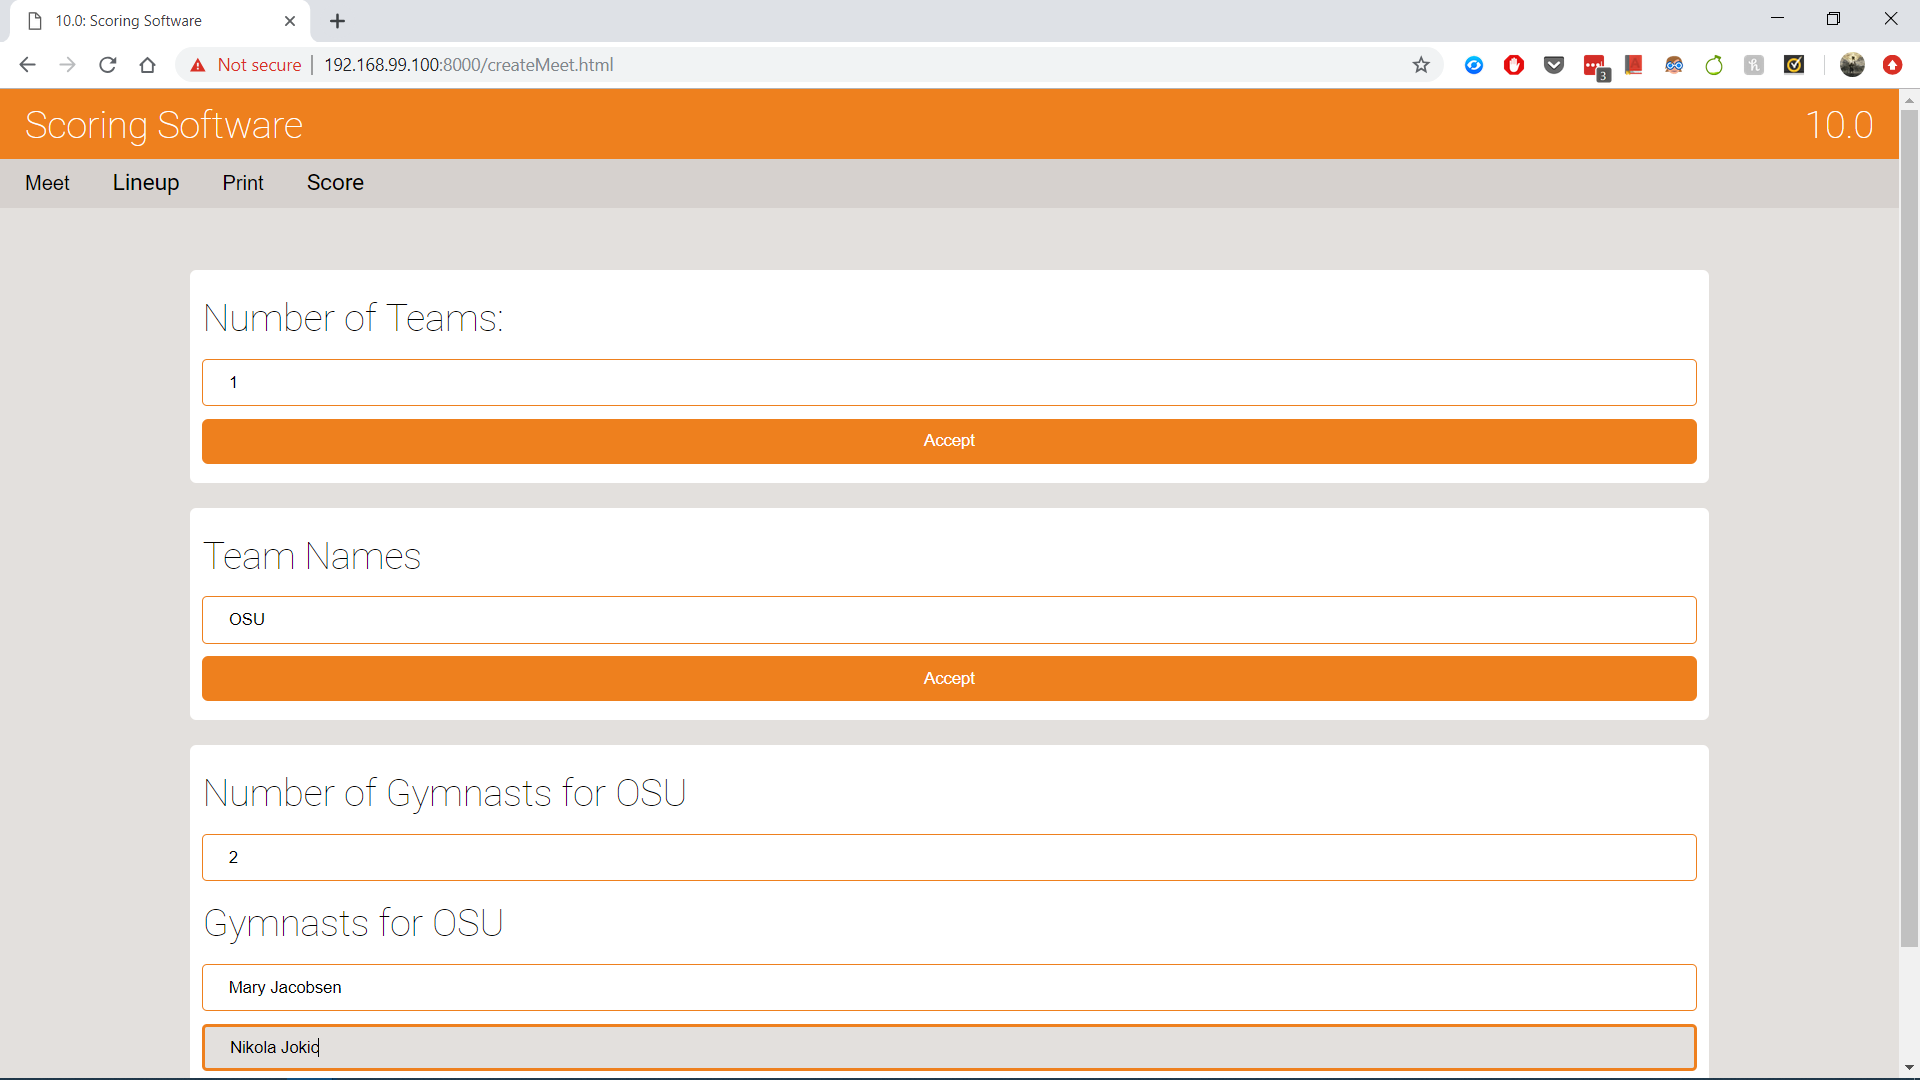
\includegraphics[width=\textwidth]{Capture.PNG}
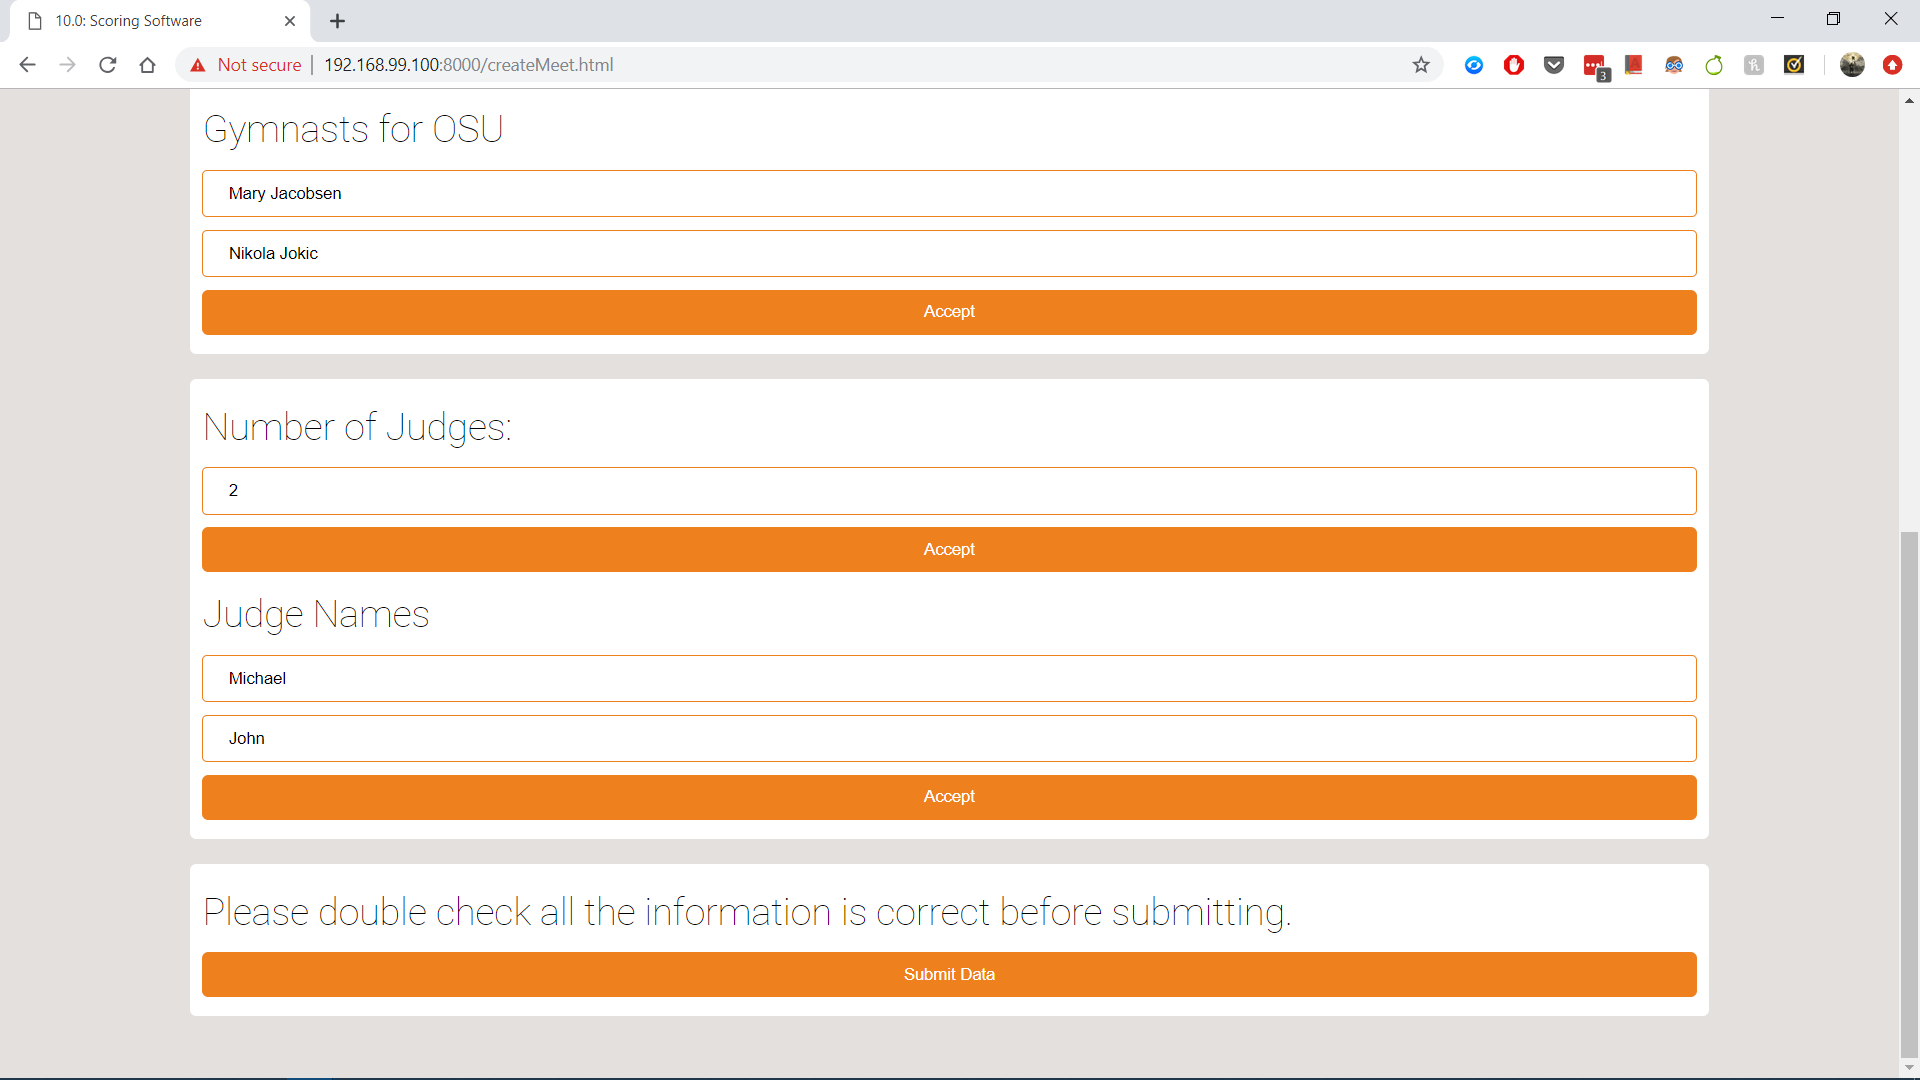
\includegraphics[width=\textwidth]{Capture2.PNG}
This page is the "Create Meet" page. The user enters the number of teams, team names, gymnast names for each team, number of judges, and judge names. There is an accept button for every input field because team names, gymnast names, and judge names all depend on number of teams, number of gymnasts, and number of judges respectively. The create meet page must be filled out in order to use the lineup, score, and print pages. 
\subsection{Lineup page}
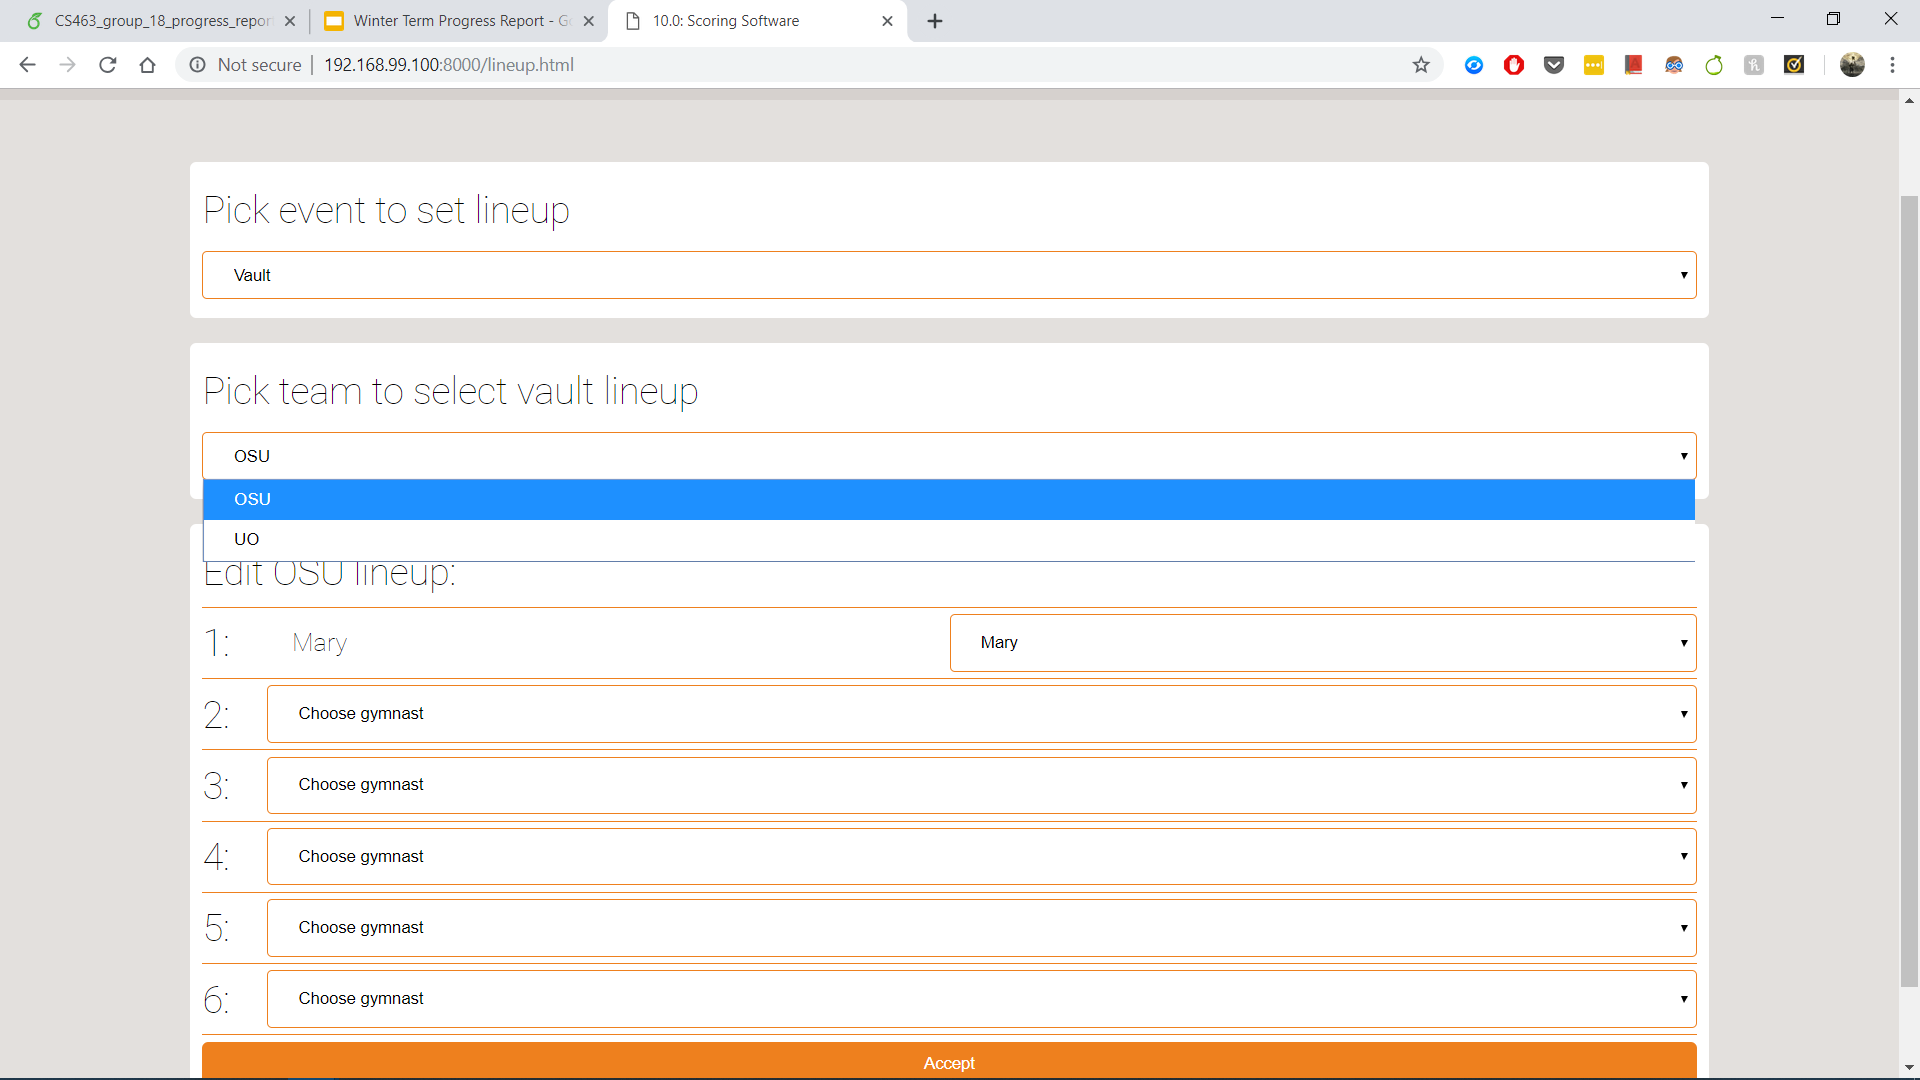
\includegraphics[width=\textwidth]{Capture3.PNG}
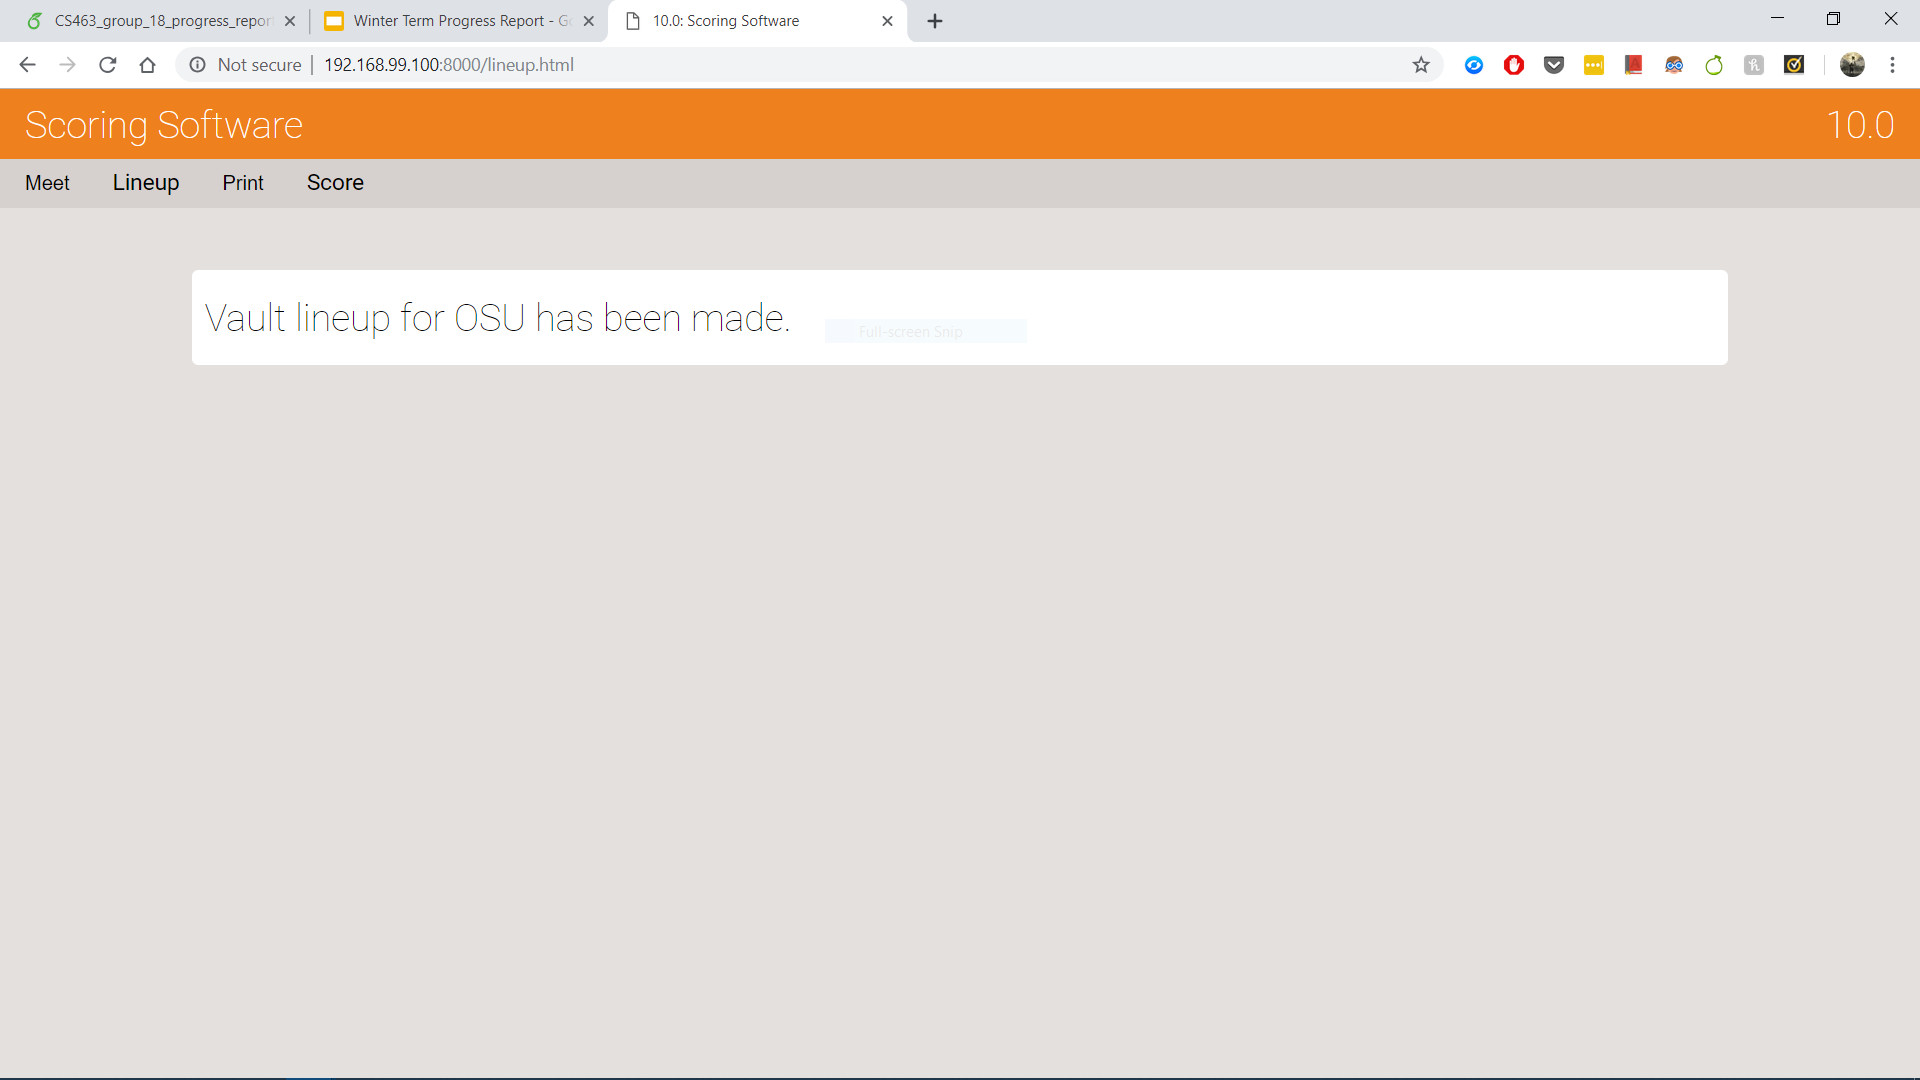
\includegraphics[width=\textwidth]{Capture4.PNG}
This is the lineup page. First, the user selects which event to set the lineups for. Then, the user chooses the team to set the lineups for. Finally, the user can set the lineup of that team for the chosen event. After the lineup is set, the user will see a confirmation page.
\subsection{Score page}
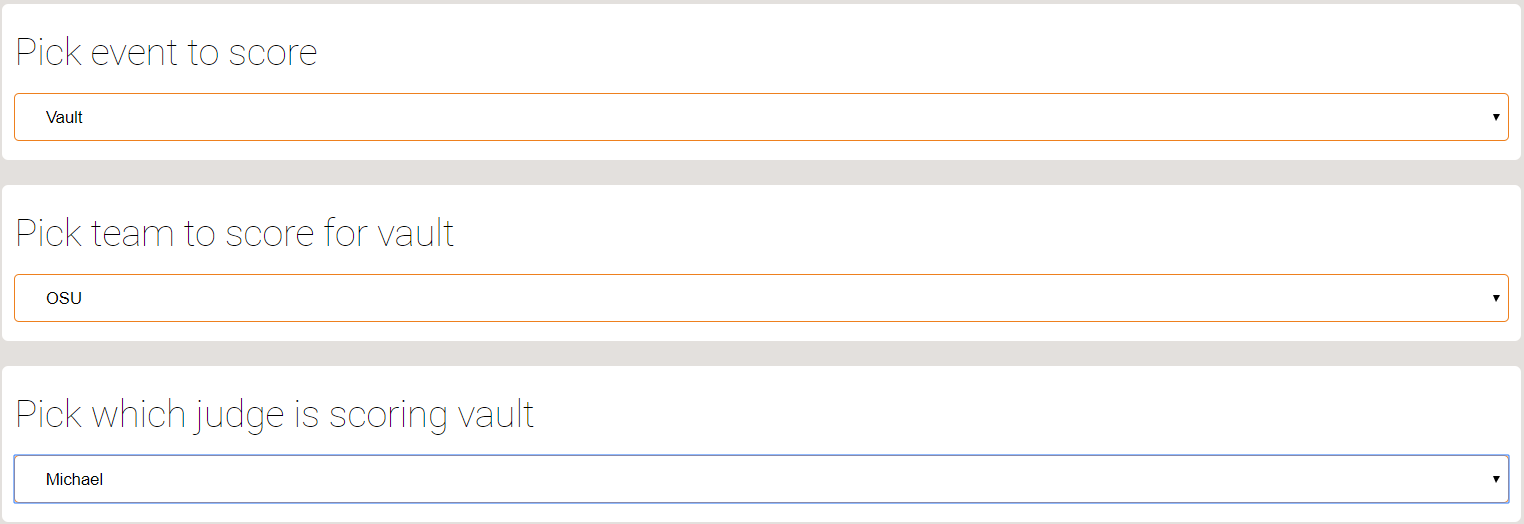
\includegraphics[width=\textwidth]{Capture5.png}
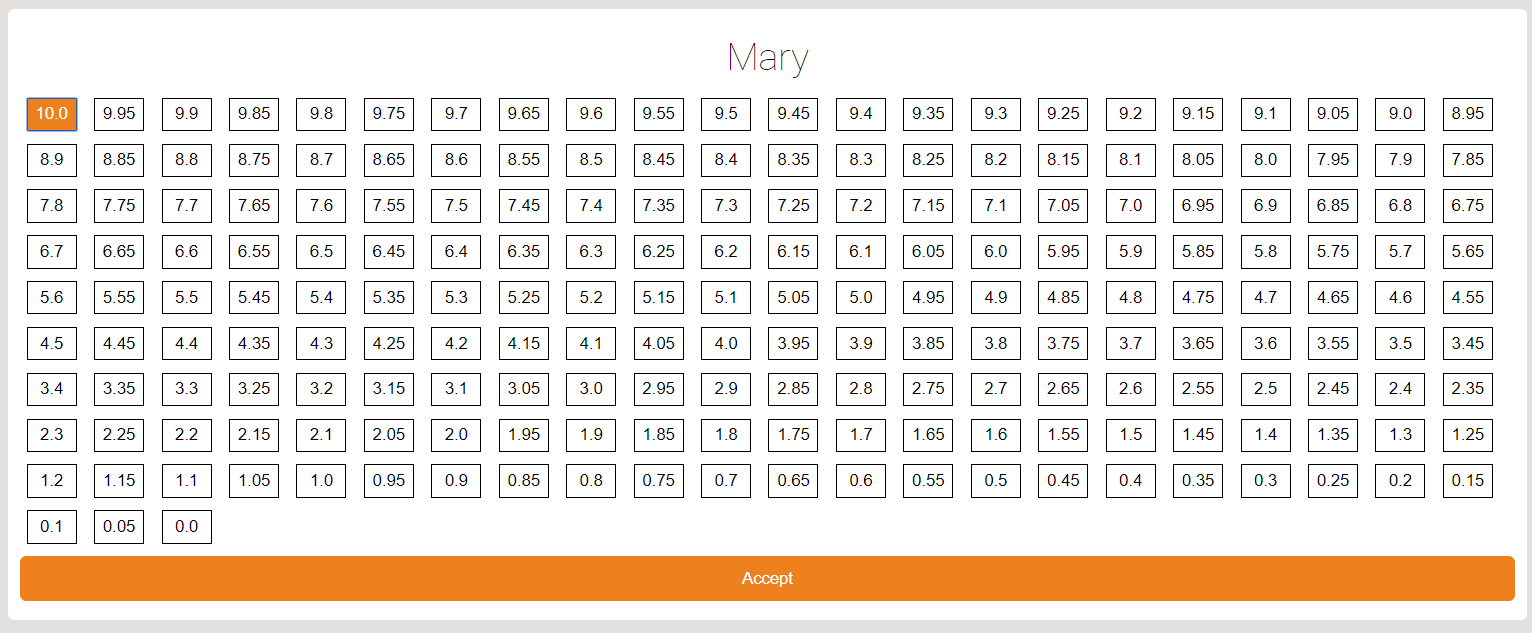
\includegraphics[width=\textwidth]{Capture6.png}
This is the score page. The user chooses an event to score and the team to score. Then, the web application displays one player at a time (from the selected team) to score for that event. The user must assign a score between 0 and 10 in increments of 0.05. After the user successfully finishes the scoring, the user will see a confirmation page.

\includegraphics[width=\textwidth]{Capture8.png}
\end{document}
